\documentclass{article}

\usepackage{arxiv}

\usepackage{hyperref}       % hyperlinks
\usepackage{url}            % simple URL typesetting
\usepackage{amsfonts}       % blackboard math symbols
\usepackage{amsmath}
\usepackage{nicefrac}       % compact symbols for 1/2, etc.
\usepackage{graphicx}
\usepackage{natbib}
\usepackage{csquotes}


\title{Dark energy is due to a math error from 1930}

\date{\today}

\author{
  \href{https://orcid.org/0000-0001-6450-3262}{
\includegraphics[scale=0.06]{orcid.pdf}\hspace{1mm}Logan P.~Evans}
  \\ \texttt{loganpevans@gmail.com}
}

% Uncomment to override  the `A preprint' in the header
%\renewcommand{\headeright}{Technical Report}
%\renewcommand{\undertitle}{Technical Report}
\renewcommand{\shorttitle}{\textit{arXiv} Template}

\hypersetup{
pdftitle={Dark energy is due to a math error from 1935},
pdfsubject={astro-ph.CO},
pdfauthor={Logan P.~Evans},
pdfkeywords={cosmological parameters, dark energy},
}

\begin{document}
\maketitle

\begin{abstract}
  Observations of distant objects, such as supernovae and galaxies, is dimmed
  due to three phenomena associated with redshift: energy levels per photon,
  spectral bandwidth, and time dilation. Observed magnitudes are reported with
  k-corrections that should correct for these dimming effects, but since 1935,
  the equations used to perform these k-corrections have been missing the
  correction factor for time dilation. When observations of Type Ia supernova
  are corrected for this missing factor, the relationship between luminosity
  distance and redshift for Type Ia supernova becomes linear. This indicates
  that the expansion rate of the universe is not accelerating and there is no
  need for dark energy to explain observational data.
\end{abstract}

% keywords can be removed
\keywords{Cosmological Parameters \and Dark Energy \and Luminosity Distance}

\section{Introduction}

Observations of Type Ia supernova are fundamental to the study of cosmology.
These measurements are necessary to calibrate models that measure redshift and
estimate distance. This relationship, often called the Hubble-Lema\^{i}tre law,
[TODO: find citation] describes how quickly the universe is expanding. However,
\citet{riess1998} and \citet{perlmutter1999} presented evidence that there
isn't a linear relationship between redshift and distance, but instead, distant
objects are father away than their redshift would predict (see Figure
\ref{fig:mu_distance_vs_redshift}). This phenomenon, whatever its source, is
referred to as dark energy.

Type Ia supernova are used to explore the relationship between distances and
redshifts because these events always happen in similar ways, so the absolute
brightness is roughly always the same. An analogy is to imagine someone walking
in the dark and lighting matches. As long as we know how brightly a match burns
at a known distance, we can estimate the distance to any match by measuring the
appearant brightness before applying some geometry.

It turns out that measuring the apperant brightness of a Type Ia supernova is
non-trivial. The aspect of the process that we will explore here concerns how
redshift affects the light we observe. This problem is often referred to as
k-corrections, and one of the first mathematical treatments of the problem was
performed by \citet{desitter1934}.

Willem de Sitter recognized three issues that would reduce the observed
magnitude of a distant observation. First, a redshifted photon carries less
energy than when it was originally emitted. Second, a narrow spectrum of
emitted light will be spread out over a larger observed spectrum. Finally, time
dilation will reduce the rate at which an observer detects photons. The
correction for each of these issues is identical: take a measurement and
multiply it by the factor $1 + z$.

A year later, \citet{hubble1935} published a similar set of calculations for
k-corrections, but these equations used $(1 + z)^2$ instead of the $(1 + z)^3$
correction term used by de Sitter. The Hubble k-corrections have been used ever
since.

Hubble and de Sitter were clearly aware of all three dimming effects associated
with redshift, but by \citet{oke1968energy}, the two factors of $(1 + z)$ were
attributed to the change in energy and to the spectral bandwidth elongation,
which leaves time dilation as the factor that was omitted.

In 1935, the correction of $(1 + z)^2$ empirically lined up the data so that
there seemed to be a linear relationship between redshift and distance. It
wasn't until \citet{riess1998}, sixty-three years later, that the omission of a
third $(1 + z)$ correction factor resulted in faulty conclusions.

Those faulty conclusions, however, have been the basis for a substantial amount
of scientific interest. In 2011, three physicists received the Nobel Prize in
Physics for discovering that the expansion rate of the universe is accelerating
\citet{straumann2012}. The papers \citet{riess1998} and \citet{perlmutter1999}
have each received over 20000 citations. It's not clear how much cosmology work
will need to be revisited with corrected distance measurements, but it is a
non-trivial amount.

\begin{displayquote}
\end{displayquote}

\section{The dimming effects of redshift}

The magnitude measurements for Type Ia supernova goes through a long chain of
data processing. The data used here was collected by the Dark Energy Survey
Collaboration, as summarized in \citet{abbott2024} and described in more detail
by \citet{vincenzi2024}. However, the data processing does not explicitly
correct for either redshift or time dilation.

In the big bang model, there are multiple phenomena associated with redshift that we
might expect to reduce the apparent magnitude of a Type Ia supernova.

\subsection{Recessional velocity redshift}

The energy carried by a photon is inversely proportional to wavelength, given
by the Planck relation

\begin{equation}
  E = \frac{hc}{\lambda}
\end{equation}

where $E$ is energy, $h$ is the Planck constant, $c$ is the speed of light, and
$\lambda$ is the wavelength.

As redshift increases the wavelength of a photon, the energy decreases.

The supernova data collected by the DES Collaboration used a CCD camera, a
photon counting device, as described by \citet{flaughter2015}.  \citet{kim1996}
noted that photometric measurements that depend on bolometers will need to be
corrected for the reduced energy level of redshifted light, but with a photon
counting device, this correction is not necessary.

While the redshift phenomenon should impact the light detected from distant
supernova, it should not impact the magnitude measurements so it does not need
to be explicitly corrected.

\subsection{Time dilation}

The second phenomenon is that time dilation for objects moving quickly relative
to our observational rest frame will reduce the rate at which photons are being
emitted. Instead of changing the properties of individual photons, time
dilation reduces the count of photons by a factor of $\frac{1}{1+z}$ where $z$
is the redshift.

This phenomenon will not be addressed by the nuances of any measuring device,
so it must be explicitly corrected.

\subsection{Stretching of space}

If space itself is stretching, it will both increase the wavelength of photons
and also reduce the density of those photons. If space is stretching at a
constant rate, the effect would be indistinguishable from the redshift and time
dilation created by high relative recessional velocities. However, an
accelerating expansion of the universe may indicate a non-constant rate of
stretching. This would manifest by distant objects having a greater distance
per redshift than nearby objects.

This non-linear streching-of-space model would be indistinguishable from a
scenario where a constant force is pushing all objects away from each other.

\subsection{Tired light}

An alternative to the big bang theory is the tired light hypothesis, as
described by \citet{zwicky1929} and \citet{shao2013}. The idea is that distant
objects are mostly stationary relative to us, but the energy of light is lost
as it travels through space. A feature of the tired light hypothesis is that
since distant objects do not have a high relative velocity to us, they should
not show time dilation.

However, as shown by \citet{blonden2008} and \citet{white2024}, distant
supernova do experience time dilation. Based on this, we can reject the tired
light hypothesis and assume the big bang model.

\section{Correcting magnitude for time dilation}

Luminosity distance $D_L$, is the apparent distance of an object based on the
observed luminosity, also known as the flux $F$. This does not take into
account any movement of the observed object between the time when the light was
emitted and the light is observed.

To derive the luminosity distance from these measurements, we start
by computing the flux $F$. Magnitude $m$ is defined on a logarithmic scale
where magnitude 1 has 100 times the brightness of magnitude 6, leading to

\begin{equation}
  F = \frac{1}{\sqrt[5]{100}^{m - 1}}.
\end{equation}

This is proportional to the number of photons detected by a telescope. We can
find the corrected flux $F^*$ by multiplying by $k(z)$, the redshift correction
factor. Time dilation of quickly moving objects reduces the number of photons
by a factor of $\frac{1}{1 + z}$, so we have

\begin{equation}
\begin{aligned}
  F^* &= F \times k(z) \\
      &= F (1 + z).
\end{aligned}
\end{equation}

To compute the corrected magnitude $m^*$, we can solve

\begin{equation}
\begin{aligned}
   F^* &= \frac{1}{\sqrt[5]{100}^{m^* - 1}} \\
   m^* &= m - \frac{\ln{(z + 1)}}{\ln{(\sqrt[5]{100})}}.
\end{aligned}
\end{equation}

From here, we can use the standard distance modules $\mu$ defined as

\begin{equation}
  \mu = m^* - M
\end{equation}

where $M$ is the absolute magnitude. The luminosity distance $D_L$ in parsecs
can then be calculated as

\begin{equation}
  D_L = 10^{1 + \frac{\mu}{5}}.
\end{equation}

\section{Linear distance vs redshift relationship}

The theory of an accelerating expansion is based on there being a non-linear
relationship between redshift and distance. More specifically, old objects (the
ones that are more distant) should have more distance per redshift than newer
objects.

As shown in Figure \ref{fig:mu_distance_vs_redshift}, this non-linear
relationship is only observed when $k(z) = 1$, meaning that magnitude is not
corrected for time dilation.

In contrast, when $k(z) = 1 + z$, time dilation is accounted for and there is a
linear relationship between redshift and distance. A linear model rules out an
accelerated expansion.

\begin{figure}[h!]
  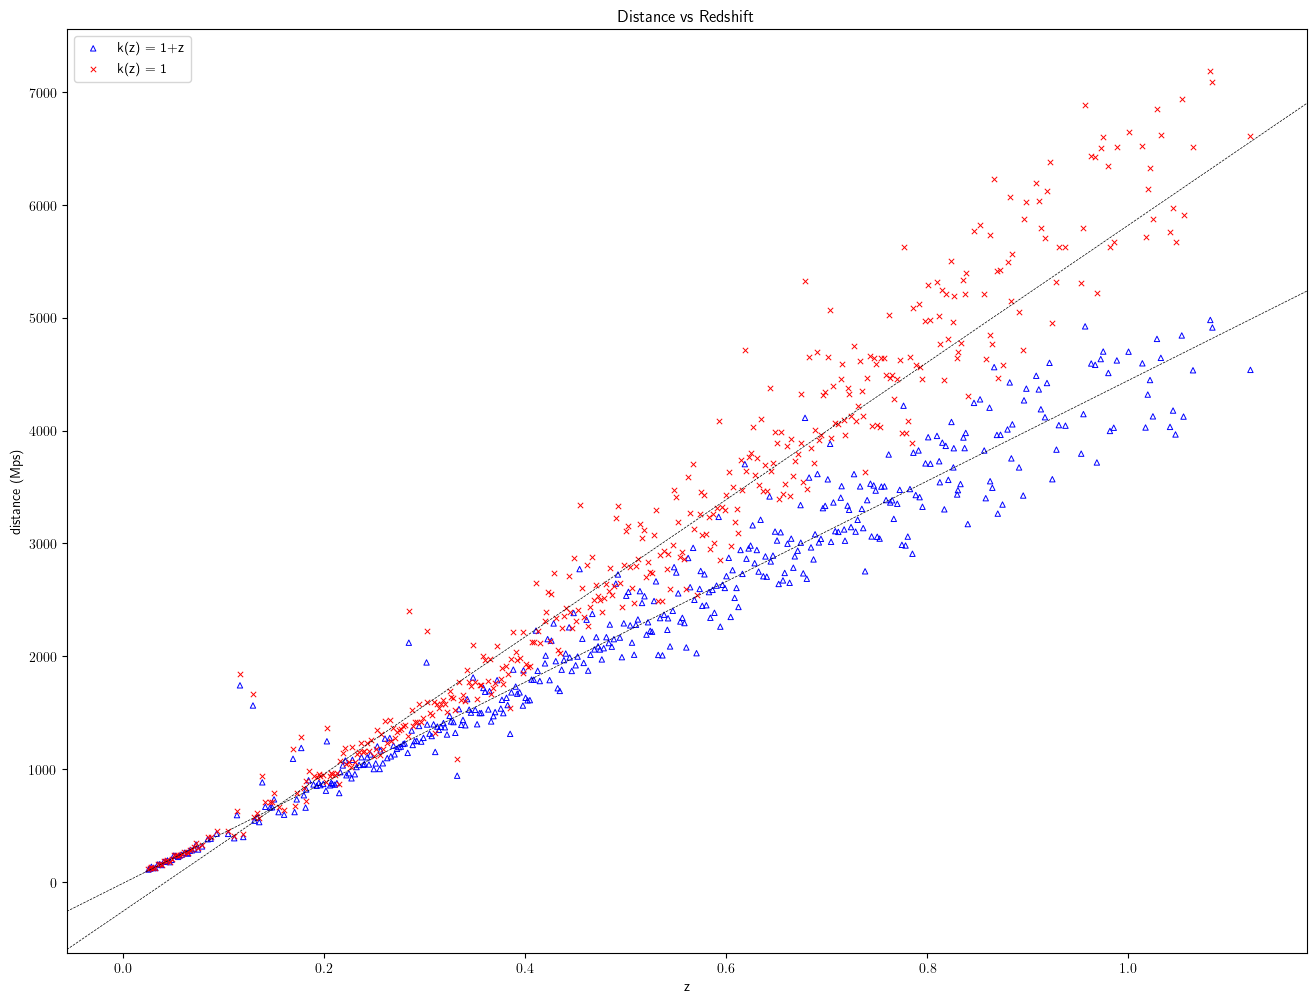
\includegraphics[width=\linewidth]{mu_distance_vs_redshift.png}
  \caption{The relationship between distance and redshift for two treatments of
  magnitude data. The displayed points are roughly a third of the values in the
  full DES dataset, selected evenly to aid visibility. The $k(z) = 1$ treatment
  is clearly non-linear while the $k(z) = 1 + z$ treatment appears to be
  linear.}
  \label{fig:mu_distance_vs_redshift}
\end{figure}

\begin{figure}[h!]
  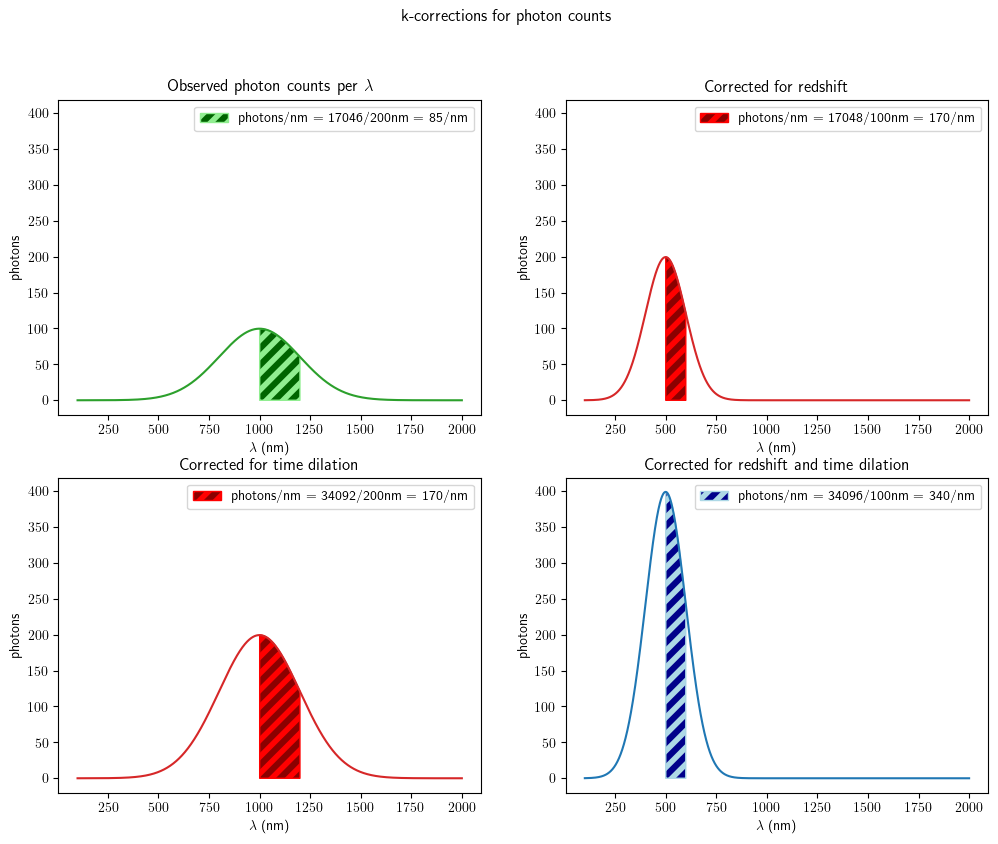
\includegraphics[width=\linewidth]{k-corrections_for_photon_counts.png}
  \caption{An example of how k-corrections take an observed spectrum and
  produce a rest-frame spectrum. [TODO]
  }
  \label{fig:mu_distance_vs_redshift}
\end{figure}

\begin{figure}[h!]
  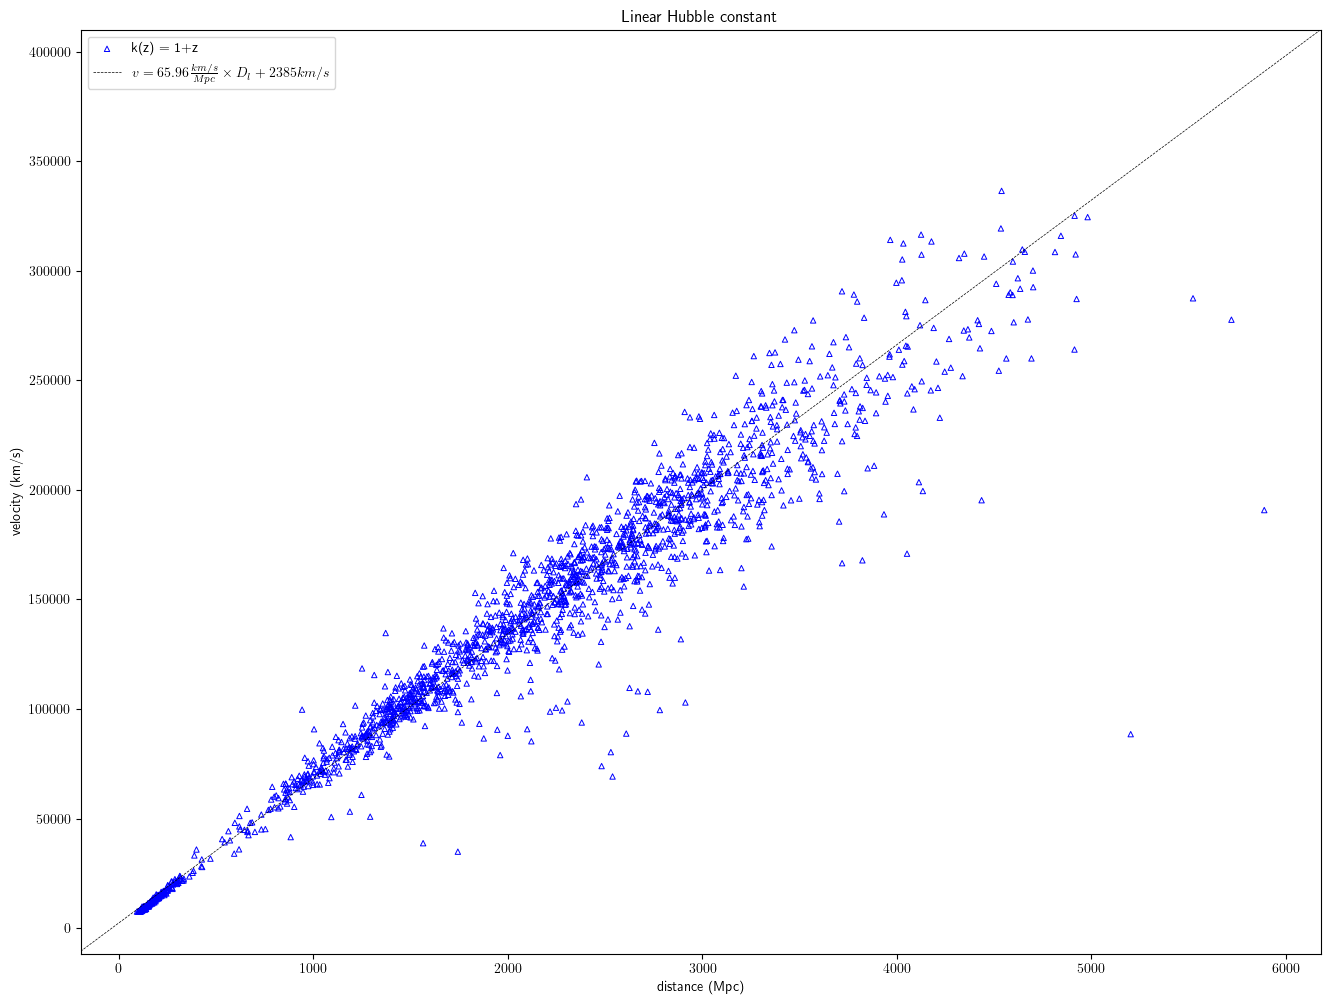
\includegraphics[width=\linewidth]{velocity_vs_distance.png}
  \caption{The relationship between expansion velocity and distance. The slope of this graph demonstrates the Hubble constant.
  }
  \label{fig:mu_distance_vs_redshift}
\end{figure}

\begin{figure}[h!]
  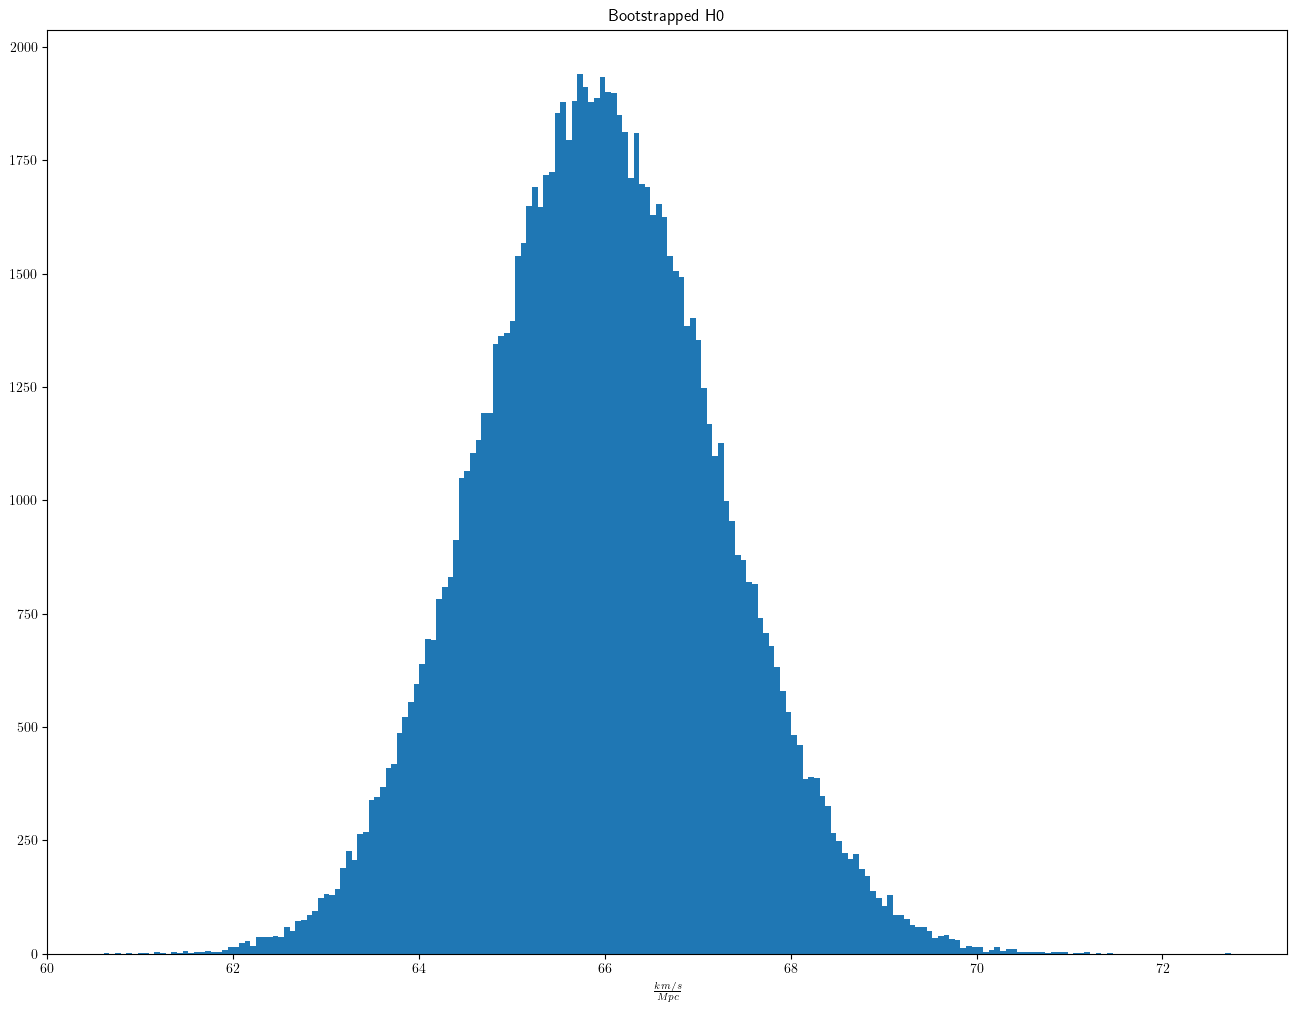
\includegraphics[width=\linewidth]{bootstrapped_H0.png}
  \caption{A histogram of 100000 bootstrap trials measuring the Hubble constant
  $H0$. Each trial samples an absolute Type Ia magnitude $M \sim Norm(-19.2334,
  0.0404)$ based on data published by \citet{camarena2020}. It then samples,
  with replacement, a population of supernovae from the dataset published by
  \citet{abbott2024}. Finally, it uses the non-parametric linear regression
  technique described by \citet{siegel1982}. The result of the bootstrap is $H0
  \sim Norm(65.94, 1.29)$.
  }
  \label{fig:mu_distance_vs_redshift}
\end{figure}

\section{Disagreement with existing research}

Previous studies use $F$ instead of $F*$. To the best of our knowledge, no
studies that depend on the distance of Type Ia supernova, reaching back at
least to \citet{kim1996}, \citet{riess1998}, and \citet{perlmutter1999}, have
accounted for time dilation.

\bibliographystyle{unsrtnat}
\bibliography{references}

\end{document}
